%%%%%%%%%%%%%%%%%%%%%%%%%%%%%%%%%%%%%%%%%
% Jacobs Landscape Poster
% LaTeX Template
% Version 1.0 (29/03/13)
%
% Created by:
% Computational Physics and Biophysics Group, Jacobs University
% https://teamwork.jacobs-university.de:8443/confluence/display/CoPandBiG/LaTeX+Poster
% 
% Further modified by:
% Nathaniel Johnston (nathaniel@njohnston.ca)
%
% This template has been downloaded from:
% http://www.LaTeXTemplates.com
%
% License:
% CC BY-NC-SA 3.0 (http://creativecommons.org/licenses/by-nc-sa/3.0/)
%
%%%%%%%%%%%%%%%%%%%%%%%%%%%%%%%%%%%%%%%%%

%----------------------------------------------------------------------------------------
%   PACKAGES AND OTHER DOCUMENT CONFIGURATIONS
%----------------------------------------------------------------------------------------

\documentclass[final]{beamer}

\usepackage[scale=1.24]{beamerposter} % Use the beamerposter package for laying out the poster

\usetheme{confposter} % Use the confposter theme supplied with this template

\setbeamercolor{block title}{fg=purple,bg=white} % Colors of the block titles
\setbeamercolor{block body}{fg=black,bg=white} % Colors of the body of blocks
\setbeamercolor{block alerted title}{fg=white,bg=dblue!70} % Colors of the highlighted block titles
\setbeamercolor{block alerted body}{fg=black,bg=dblue!10} % Colors of the body of highlighted blocks
% Many more colors are available for use in beamerthemeconfposter.sty

%-----------------------------------------------------------
% Define the column widths and overall poster size
% To set effective sepwid, onecolwid and twocolwid values, first choose how many columns you want and how much separation you want between columns
% In this template, the separation width chosen is 0.024 of the paper width and a 4-column layout
% onecolwid should therefore be (1-(# of columns+1)*sepwid)/# of columns e.g. (1-(4+1)*0.024)/4 = 0.22
% Set twocolwid to be (2*onecolwid)+sepwid = 0.464
% Set threecolwid to be (3*onecolwid)+2*sepwid = 0.708

\newlength{\sepwid}
\newlength{\onecolwid}
\newlength{\twocolwid}
\newlength{\threecolwid}
\setlength{\paperwidth}{78in} % Width (Maximun is 96 in)
\setlength{\paperheight}{43in} % Heighth (Maximun is 48 in)
\setlength{\sepwid}{0.024\paperwidth} % Separation width (white space) between columns
\setlength{\onecolwid}{0.22\paperwidth} % Width of one column
\setlength{\twocolwid}{0.464\paperwidth} % Width of two columns
\setlength{\threecolwid}{0.708\paperwidth} % Width of three columns
\setlength{\topmargin}{0in} % Reduce the top margin size
%-----------------------------------------------------------

\usepackage{graphicx}  % Required for including images
\usepackage[utf8]{inputenc}
\usepackage[portuges, brazil]{babel}   
\usepackage{booktabs} % Top and bottom rules for tables

%----------------------------------------------------------------------------------------
%   TITLE SECTION 
%----------------------------------------------------------------------------------------

\title{The Mirror Effect within Perception: Not another Recognition Memory Study} % Poster title

\author{Adriana F. Chávez De la Peña} % Author(s)

\institute{National Autonomous University of Mexico (UNAM); Faculty of Psychology\\ Lab 25;  PAPIIT IN} % Institution(s)

%----------------------------------------------------------------------------------------

\begin{document}

\addtobeamertemplate{block end}{}{\vspace*{1.5ex}} % White space under blocks
\addtobeamertemplate{block alerted end}{}{\vspace*{1.5ex}} % White space under highlighted (alert) blocks

\setlength{\belowcaptionskip}{2ex} % White space under figures
\setlength\belowdisplayshortskip{2ex} % White space under equations

\begin{frame}[t] % The whole poster is enclosed in one beamer frame

\begin{tikzpicture}[remember picture,overlay]
\node[anchor=north west] at ([shift={(5cm,-1cm)}]current page.north west)
    {
\includegraphics[width=10cm]{Figures/UNAMiwi.jpg}};
\node[anchor=north west] at ([shift={(23cm,-2cm)}]current page.north west)
    {
\includegraphics[width=10cm]{Figures/Psicologia.png}};
\node[anchor=north east] at ([shift={(-15cm,-1cm)}]current page.north east)
    {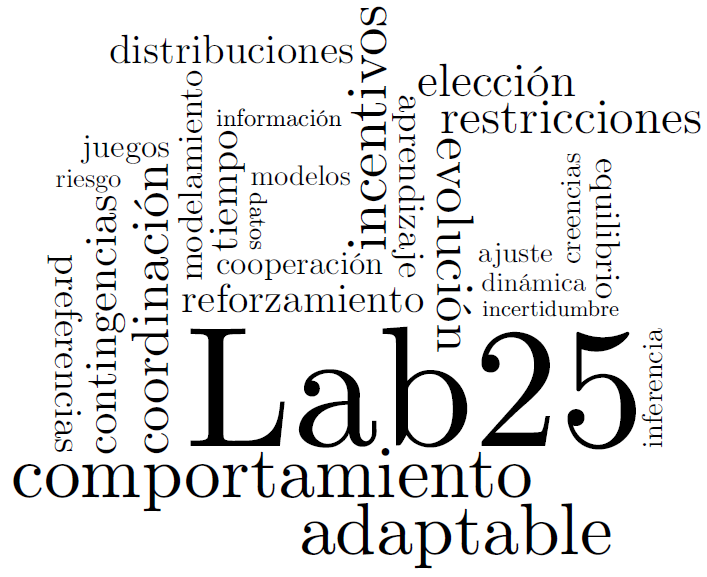
\includegraphics[width=12cm]{Figures/Lab25.png}};
\end{tikzpicture}

\begin{columns}[t] % The whole poster consists of three major columns, the second of which is split into two columns twice - the [t] option aligns each column's content to the top

\begin{column}{\sepwid}\end{column} % Empty spacer column

\begin{column}{\onecolwid} % The first column

%----------------------------------------------------------------------------------------
%   OBJECTIVES
%----------------------------------------------------------------------------------------

%\begin{alertblock}{Abstract}

%Within recognition memory studies where Signal Detection Theory has been applied to describe subjects’ performance, a pattern of responses known as the Mirror Effect has shown that when comparing subjects’ performance between classes of stimuli that are differentially recognized, this difference appears both for the identification of known and new items. However, the extensiveness of this pattern to other fields has not been explored yet. By using what is known about the Ebbinghaus illusion to design two levels of discriminability, evidence of the Mirror Effect in a detection task, confidence ratings included, that involves perception only is shown.

%\begin{itemize}
%\item Mollis dignissim, magna augue tincidunt dolor, interdum vestibulum urna
%\item Sed aliquet luctus lectus, eget aliquet leo ullamcorper consequat. Vivamus eros %sem, iaculis ut euismod non, sollicitudin vel orci.
%\item Nascetur ridiculus mus.  
%\item Euismod non erat. Nam ultricies pellentesque nunc, ultrices volutpat nisl ultrices a.
%\end{itemize}

%\end{alertblock}

%----------------------------------------------------------------------------------------
%   INTRODUCTION
%----------------------------------------------------------------------------------------

\begin{alertblock}{Introduction}

Signal detection theory has been applied to Recognition Memory to describe subjects’ ability to discriminate between stimuli that have previously been presented (old stimuli) from a new set of stimuli (Wixted, 2007). Within this field a consistent pattern of responses, identified as the Mirror Effect, has appeared when subjects’ hit and false alarm rates are compared between two classes of stimuli, one being more easily recognized (A) than the other (B), this difference is supported by discrepancies in the identification of both, old and new items, (Glanzer, Adams, Kim, 1993). 



\begin{figure}
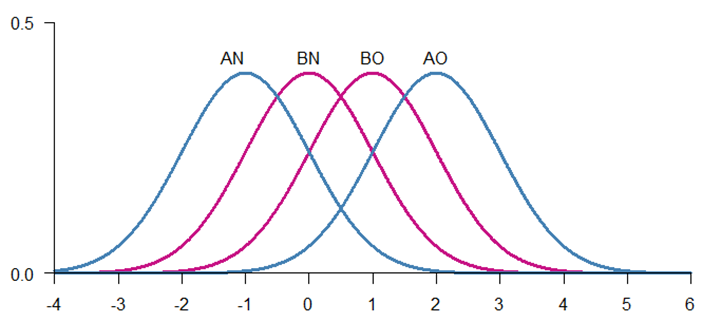
\includegraphics[width=0.6\linewidth]{Figures/MirrorEffect.png}
\end{figure}




Evidence in favor of the Mirror Effect has been reported across a wide range of variables influencing stimuli recognition and several SDT-alike procedures:



In typical Yes/No tasks, the Mirror Effect appears as:


\begin{equation}
FalseAlarms(A) < FalseAlarms(B) < Hits(B) < Hits(A)
\label{eqn:Rates}
\end{equation}



The pattern also appears when participants are asked to valuate how confident they felt while answering to each trial, giving the following mean confidence-rating pattern for Affirmative answers (a.k.a. -Yes, I've seen it before-).



\begin{equation}
R(AN) < R(BN) < R(BS) < R(AS)
\label{eqn:Confidence}
\end{equation}




Surprisingly, evidence for the Mirror Effect has only been collected within Recognition Memory studies. Thus, most theories and models proposed to explain this pattern tend to do it in terms of high-level processes engaged in the study phase, where subjects interact for the first time with the stimuli and, presumably, attend/process them differently, leading to the different rates of response observed in the recognition phase, (DeCarlo, 2007, Glanzer et. al, 1993). 












The main goal of the present study was to explore the existence of the Mirror Effect outside Recognition Memory to test the assumption that it depends on high-level processing differences engaged during a study phase. Therefore, we constructed a detection task that involves perception only, and uses a largely studied optical illusion, the Ebbinghaus circles, to design to levels of discriminability.




\end{alertblock}

%------------------------------------------------

%\begin{figure}
%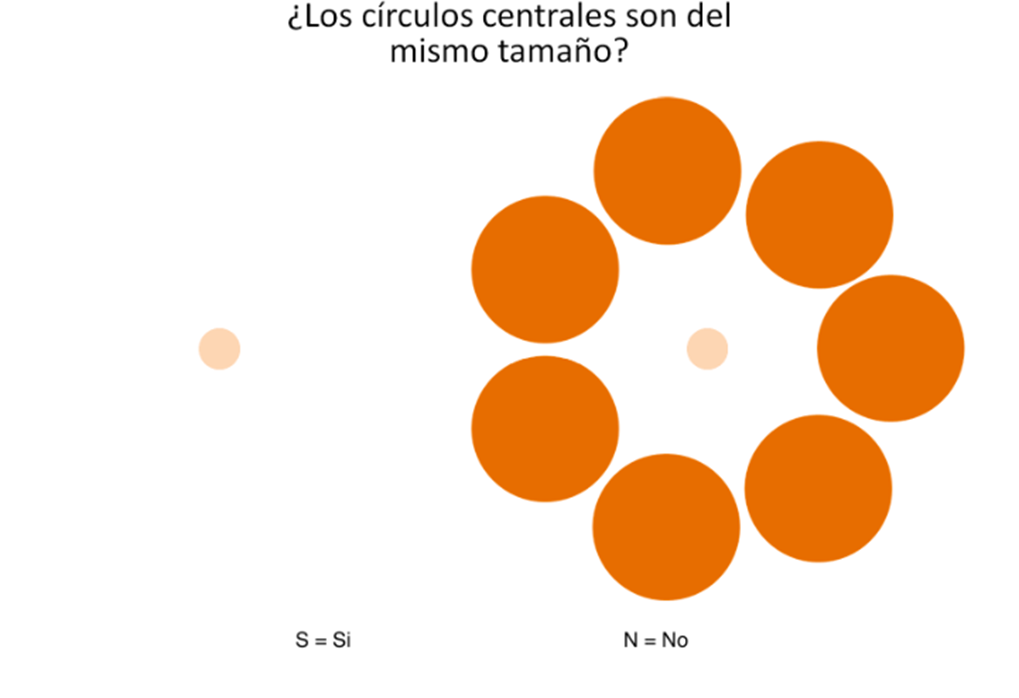
\includegraphics[width=1\linewidth]{Figures/MainTask.png}
%\caption{Figure caption}
%\end{figure}

%----------------------------------------------------------------------------------------

\end{column} % End of the first column

\begin{column}{\sepwid}\end{column} % Empty spacer column

\begin{column}{\twocolwid} % Begin a column which is two columns wide (column 2)

\begin{columns}[t,totalwidth=\twocolwid] % Split up the two columns wide column

\begin{column}{\onecolwid}\vspace{-.6in} % The first column within column 2 (column 2.1)

%----------------------------------------------------------------------------------------
%   MATERIALS
%----------------------------------------------------------------------------------------

\begin{block}{Method}

Two levels of perceptual discriminability were constructed according to the literature on the variables involved in the Ebbinghaus illusion, where the number of external circles has shown to be directly related to the intensity of the illusion (Massaro, 1971).




\begin{itemize}
\item High accuracy (A): Ebbinghaus illusions with 2 or 3 surrounding circles.
\item Low accuracy (B): Ebbinghaus illusions with 7 or 8 surrounding circles.
\end{itemize}



Detection task:  Are the two central circles of the same size?

Two experiments: 

\begin{itemize}
\item Experiment 1: Just the right circle to compare is shown part of an Ebbinghaus illusion.
\item Experiment 2: Both circles were constructed as Ebbinghaus illusions.
\end{itemize}


ether two circles appearing on screen were the same size (Signal) or not (Noise); these circles were presented on a bright color and identified by the name of ‘central circles’. In Experiment 1 both circles were constructed as Ebbinghaus illusions, varying the number of surrounding circles on each trial.
Experiment 2 consisted of a single Ebbinghaus illusion-circle that had to be compared with an aisle, constant, reference circle. Both experiments included underestimation and overestimation-inducing Ebbinghaus illusion.
Each experiment included a total of 640 trials (320 trials for each class of stimuli, A or B, with 120 signal and noise trials respectively) presented at random. On each trial, stimuli were shown for only 1.5 seconds to prevent habituation to the illusion. Participants could enter their response (‘Yes, circles are the same size’ or ‘No, they’re not’) either before or after stimuli disappeared from screen.
After the first response was given, a scale containing numbers from 1 to 3 was presented to indicate participants to grade how confident they were from their previous response by pressing one of the three possible response keys, (1-Low, 2-Medium, 3-High). However, the program registered these responses as part of a larger continuum going from 1 to 6, distinguishing ‘yes’ from ‘no’ responses:
a) If participants chose ‘No’ and pressed 3, it would be registered as 1 (Very sure noise), and so on.
b) If participants chose ‘Yes’ first and pressed 3, it would be registered as 6 (Very sure signal), and so on.
Participants had to press the space bar to indicate that they were ready to move from trial to trial. Response time was also registered.


%The materials were prepared according to the steps outlined below:
%\begin{enumerate}
%\item Curabitur pellentesque dignissim
%\item Eu facilisis est tempus quis
%\item Duis porta consequat lorem
%\item Curabitur pellentesque dignissim
%\end{enumerate}

\end{block}

%----------------------------------------------------------------------------------------

\end{column} % End of column 2.1

\begin{column}{\onecolwid}\vspace{-.6in} % The second column within column 2 (column 2.2)

%----------------------------------------------------------------------------------------
%   METHODS
%----------------------------------------------------------------------------------------

\begin{block}{Procedure}

\begin{center}
\begin{tabular}{ccc}
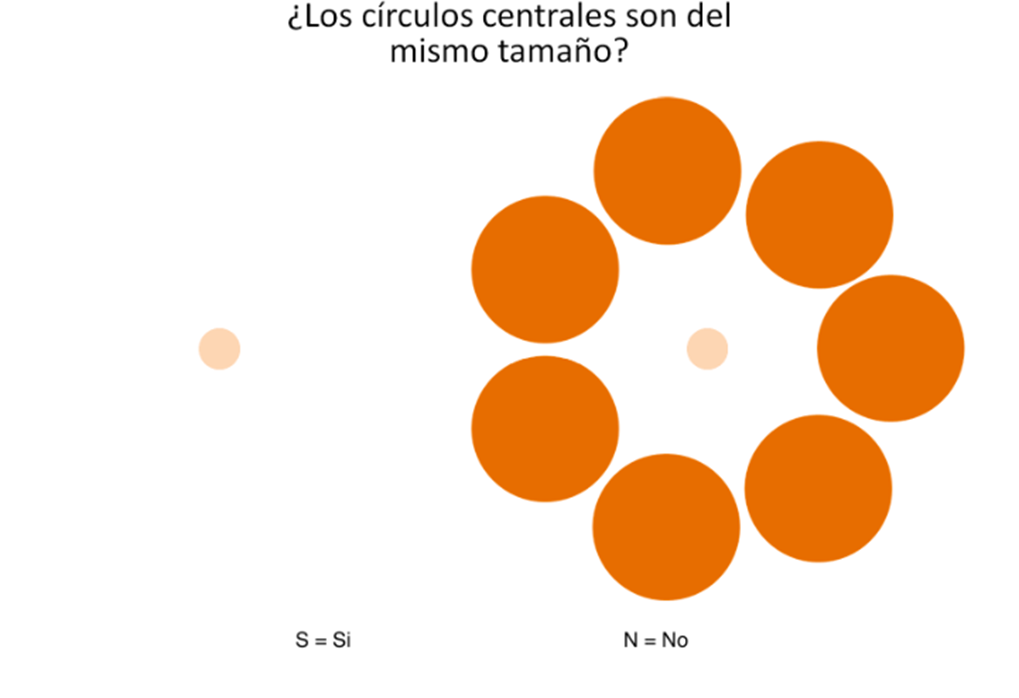
\includegraphics[width=0.55\linewidth]{Figures/MainTask.png} & \hfill & 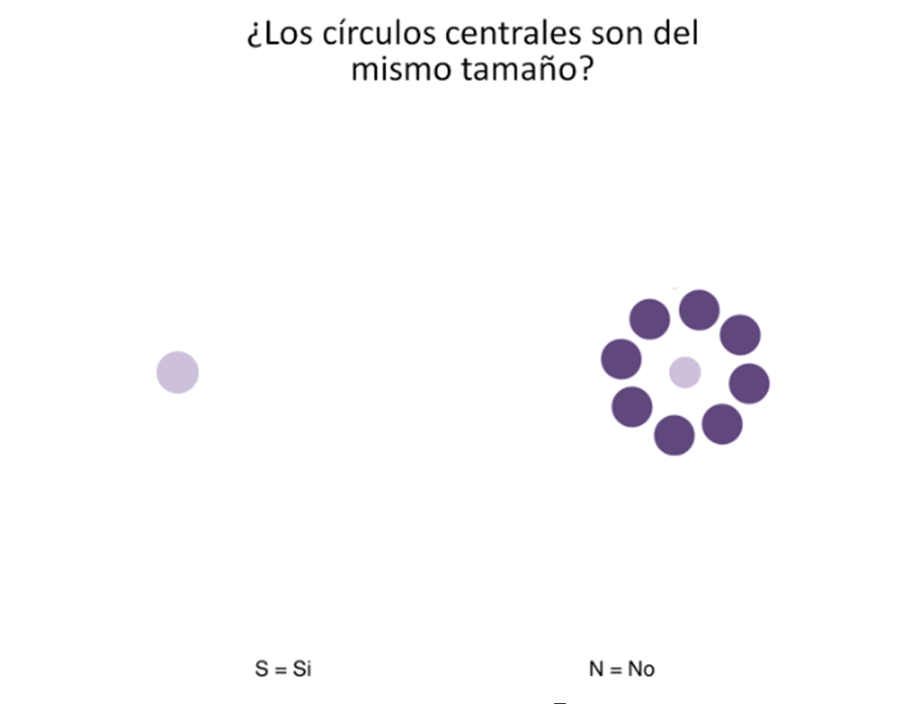
\includegraphics[width=0.5\linewidth]{Figures/MainTask2.png}
\end{tabular}
\end{center}


%Lorem ipsum dolor \textbf{sit amet}, consectetur adipiscing elit. Sed laoreet accumsan mattis. Integer sapien tellus, auctor ac blandit eget, sollicitudin vitae lorem. Praesent dictum tempor pulvinar. Suspendisse potenti. Sed tincidunt varius ipsum, et porta nulla suscipit et. Etiam congue bibendum felis, ac dictum augue cursus a. \textbf{Donec} magna eros, iaculis sit amet placerat quis, laoreet id est. In ut orci purus, interdum ornare nibh. Pellentesque pulvinar, nibh ac malesuada accumsan, urna nunc convallis tortor, ac vehicula nulla tellus eget nulla. Nullam lectus tortor, \textit{consequat tempor hendrerit} quis, vestibulum in diam. Maecenas sed diam augue.

\end{block}

%----------------------------------------------------------------------------------------

\end{column} % End of column 2.2

\end{columns} % End of the split of column 2 - any content after this will now take up 2 columns width

%----------------------------------------------------------------------------------------
%   IMPORTANT RESULT
%----------------------------------------------------------------------------------------

\begin{alertblock}{What did we find? (Spoiler alert!)}

In both experiments, the pattern of responses identified as the Mirror Effect was found on at least 85\% of the participants.

\end{alertblock} 

%----------------------------------------------------------------------------------------

\begin{columns}[t,totalwidth=\twocolwid] % Split up the two columns wide column again

\begin{column}{\onecolwid} % The first column within column 2 (column 2.1)

%----------------------------------------------------------------------------------------
%   MATHEMATICAL SECTION
%----------------------------------------------------------------------------------------

\begin{block}{Classical Data Analysis}

Nam quis odio enim, in molestie libero. Vivamus cursus mi at nulla elementum sollicitudin. Nam quis odio enim, in molestie libero. Vivamus cursus mi at nulla elementum sollicitudin.
  
\begin{equation}
E = mc^{2}
\label{eqn:Einstein}
\end{equation}

Nam quis odio enim, in molestie libero. Vivamus cursus mi at nulla elementum sollicitudin. Nam quis odio enim, in molestie libero. Vivamus cursus mi at nulla elementum sollicitudin.

\begin{equation}
\cos^3 \theta =\frac{1}{4}\cos\theta+\frac{3}{4}\cos 3\theta
\label{eq:refname}
\end{equation}

Nam quis odio enim, in molestie libero. Vivamus cursus mi at nulla elementum sollicitudin. Nam quis odio enim, in molestie libero. Vivamus cursus mi at nulla elementum sollicitudin.

\begin{equation}
\kappa =\frac{\xi}{E_{\mathrm{max}}} %\mathbb{ZNR}
\end{equation}

\end{block}

%----------------------------------------------------------------------------------------

\end{column} % End of column 2.1

\begin{column}{\onecolwid} % The second column within column 2 (column 2.2)

%----------------------------------------------------------------------------------------
%   RESULTS
%----------------------------------------------------------------------------------------

\begin{block}{Results}

\begin{figure}

\includegraphics[width=0.8\linewidth]{placeholder.jpg}
\caption{Figure caption}
\end{figure}

Nunc tempus venenatis facilisis. Curabitur suscipit consequat eros non porttitor. Sed a massa dolor, id ornare enim:

\begin{table}
\vspace{2ex}
\begin{tabular}{l l l}
\toprule
\textbf{Treatments} & \textbf{Response 1} & \textbf{Response 2}\\
\midrule
Treatment 1 & 0.0003262 & 0.562 \\
Treatment 2 & 0.0015681 & 0.910 \\
Treatment 3 & 0.0009271 & 0.296 \\
\bottomrule
\end{tabular}
\caption{Table caption}
\end{table}

\end{block}

%----------------------------------------------------------------------------------------

\end{column} % End of column 2.2

\end{columns} % End of the split of column 2

\end{column} % End of the second column

\begin{column}{\sepwid}\end{column} % Empty spacer column

\begin{column}{\onecolwid} % The third column

%----------------------------------------------------------------------------------------
%   CONCLUSION
%----------------------------------------------------------------------------------------

\begin{block}{Conclusion}

The present study is the first to show evidence for the existence of the Mirror Effect patterns of response, on a signal detection task that does not involve recognition memory. The perceptual task here presented lacked of a pre-experimental phase where participants had the chance to manipulate how powerful the illusions included in each condition were, contradicting what has been proposed within recognition memory studies. The fact that the Mirror Effect was found on a perceptual task, with accuracy conditions designed specifically in terms of the signal that participants are asked to detect, may suggest that there’s a much more basic principle regulating the patterns of response observed.

%Nunc tempus venenatis facilisis. \textbf{Curabitur suscipit} consequat eros non porttitor. Sed a massa dolor, id ornare enim. Fusce quis massa dictum tortor \textbf{tincidunt mattis}. Donec quam est, lobortis quis pretium at, laoreet scelerisque lacus. Nam quis odio enim, in molestie libero. Vivamus cursus mi at \textit{nulla elementum sollicitudin}.

\end{block}

%----------------------------------------------------------------------------------------
%   ADDITIONAL INFORMATION
%----------------------------------------------------------------------------------------

\begin{block}{Additional Information}

Maecenas ultricies feugiat velit non mattis. Fusce tempus arcu id ligula varius dictum. 
\begin{itemize}
\item Curabitur pellentesque dignissim
\item Eu facilisis est tempus quis
\item Duis porta consequat lorem
\end{itemize}

\end{block}

%----------------------------------------------------------------------------------------
%   REFERENCES
%----------------------------------------------------------------------------------------

\begin{block}{References}

\nocite{*} % Insert publications even if they are not cited in the poster
\small{\bibliographystyle{unsrt}
\bibliography{sample}\vspace{0.75in}}

\end{block}

%----------------------------------------------------------------------------------------
%   ACKNOWLEDGEMENTS
%----------------------------------------------------------------------------------------

\setbeamercolor{block title}{fg=red,bg=white} % Change the block title color

\begin{block}{Acknowledgements}

\small{\rmfamily{First of all, }} \\

\end{block}

%----------------------------------------------------------------------------------------
%   CONTACT INFORMATION
%----------------------------------------------------------------------------------------

\setbeamercolor{block alerted title}{fg=black,bg=norange} % Change the alert block title colors
\setbeamercolor{block alerted body}{fg=black,bg=white} % Change the alert block body colors

\begin{alertblock}{Contact Information}

\begin{itemize}
\item Web: \href{http://www.university.edu/smithlab}{http://www.university.edu/smithlab}
\item Email: \href{mailto:john@smith.com}{john@smith.com}
\item Phone: +1 (000) 111 1111
\end{itemize}

\end{alertblock}

\begin{center}
\begin{tabular}{ccc}

\includegraphics[width=0.4\linewidth]{logo.png} & \hfill & 
\includegraphics[width=0.4\linewidth]{logo.png}
\end{tabular}
\end{center}

%----------------------------------------------------------------------------------------

\end{column} % End of the third column

\end{columns} % End of all the columns in the poster

\end{frame} % End of the enclosing frame

\end{document}

              